\documentclass[10pt,twocolumn,letterpaper]{article}

\usepackage{iccv}
\usepackage{times}
\usepackage{epsfig}
\usepackage{graphicx}
\usepackage{amsmath}
\usepackage{amssymb}

\DeclareMathOperator*{\argmin}{arg\,min}
\DeclareMathOperator*{\argmax}{arg\,max}
\newcommand{\SUM}{\sum\limits}
% Include other packages here, before hyperref.

% If you comment hyperref and then uncomment it, you should delete
% egpaper.aux before re-running latex.  (Or just hit 'q' on the first latex
% run, let it finish, and you should be clear).
\usepackage[pagebackref=true,breaklinks=true,letterpaper=true,colorlinks,bookmarks=false]{hyperref}

\iccvfinalcopy % *** Uncomment this line for the final submission
\def\iccvPaperID{****} % *** Enter the ICCV Paper ID here
\def\httilde{\mbox{\tt\raisebox{-.5ex}{\symbol{126}}}}

% Pages are numbered in submission mode, and unnumbered in camera-ready
\ificcvfinal\pagestyle{empty}\fi
\begin{document}

%%%%%%%%% TITLE
\title{Application of Conditional Random Field in Image Salient Object Detection\\ with Local, Regional and Global Feature Extraction}

\author{Jimmy Lin\\
Australian National University\\
Canberra, Australia\\
{\tt\small \url{linxin@gmail.com}}
% For a paper whose authors are all at the same institution,
% omit the following lines up until the closing ``}''.
% Additional authors and addresses can be added with ``\and'',
% just like the second author.
% To save space, use either the email address or home page, not both
\and
Chris-Chau-Long\\
Australian National University\\
Canberra, Australia\\
{\small\url{chris.claoue.long@gmail.com}}
}

\maketitle
% \thispagestyle{empty}

%%%%%%%%% ABSTRACT
\begin{abstract}
    Making use of OpenCV, DARWIN and MSRA datasets, we detect the saliency of by extracting local, 
    regional and global saliency feature, 
    then combine those features with pre-fitted weights derived by logistic regression.
    On top of that, the conditional random field framework is constructed to capture the spatial continuity of the saliency.
    The importance ratio between the combined unary and pairwise term is determined by cross validation.
    Based on the binary mask inferred in Conditional Random Field, we ultimately apply winner-take-all algorithm to 
    output one boxing rectangle to label the detected salient object, by which the performance of our 
    approach is evaluated. 
    %%- respectively multiscale contrast, center surround histogram, and color spatial distribution. 
\end{abstract}

%% Introduction & Related Works (1 page)
\section{Introduction}
%{{{
what? Saliency is the prominence of an object in an image.

why? Salient object detection is useful in numerous areas, for instance, in siimulating human vision by robots, augmented Reality, 3D surface reconstruction and more.

Related works?

how? Often detected by its \textbf{high contrast boundary} to its near neighbours, \textbf{distinction from its surrounds}, \textbf{intensive colour distribution} compared to all other color component in candidate image and \textbf{space continuity of saliency}. \\
%}}}

%% Formulation (1 page)
\section{Formulation}
%{{{
Given an image $I$, we want to compute the location of a salient object.

Binary labelling task -- for each pixel $x$, indicate whether it belongs to the salient object (1) or not (0). 
Thus, our objective is to have corresponding map $A$, indicating binary saliency of one pixel.

    \begin{center}
        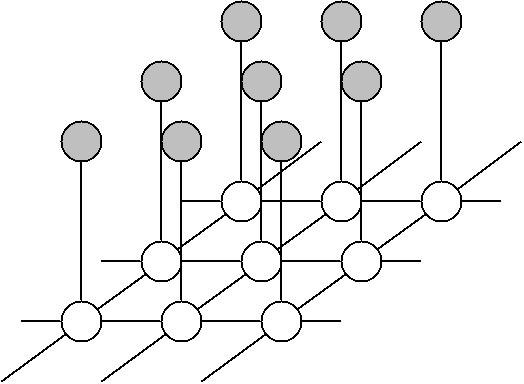
\includegraphics[width=1.8in,height=1in]{./Figures/mrf.jpg} \\
        \footnotesize Fig.2 graph for Conditional Random Field
        \end{center}

    Build up a probabilistic model $P(A|I)=\frac{1}{Z}e^{-E(A|I)}$, where $\frac{1}{Z}$ is the normalising factor, and $E(A|I)$ is the energy function incorporating both unary and pairwise potentials between pixels.

    Formally, the energy function can be represented as
    $$
    E(A|I) = \SUM_x S_{unary}(a_x,I) + \lambda_0 \SUM_{x,x'}S_{pair}(a_x,a_{x'},I)
    $$
    where $\lambda$ is the relative weight between the summary of multiple unary features and pairwise features. \\[10pt]
    The pairwise feature $S(a_x,a_{x'},I)$ exploits the spatial relationship between two adjacent pixels.  It can be viewed as a ``penalty'' for labelling adjacent pixels the same or differently.
    $$
    S(a_x,a_{x'},I) = |a_x-a_{x'}| \cdot e^{-\beta d_{x,x'}}
    $$
    where $x,x'$ represent two adjacent pixels, $d_{x,x'}$ is the L2-norm (standard norm) representing the colour difference between the two pixels, and $\beta=(2\langle||I_x-I_{x'}||^2\rangle)^{-1}$ is a robust parameter to weight the colour contrast.
    
    The unary potential for combination of three features is specified as 
    $$
    S_{unary}(a_x,I) = \SUM_{k=1}^K \lambda_k \cdot F_k(a_x,I)
    $$
    where $\lambda_k$ is the weight of the $k^{th}$ feature conforming to $\sum_{k=1}^{K} \lambda_k = 1$.
    \begin{center} %% image 5_156_156422
    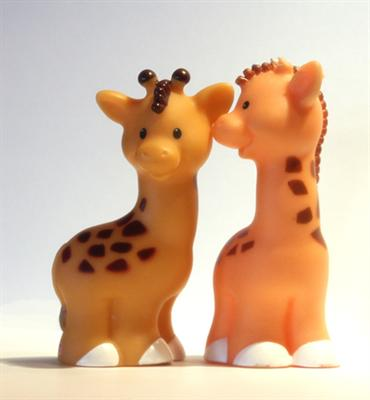
\includegraphics[width=0.6in,height=0.8in]{./Figures/previews/raw.jpg}
    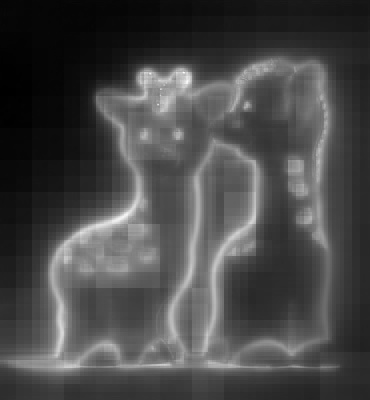
\includegraphics[width=0.6in,height=0.8in]{./Figures/previews/MC.jpg}
    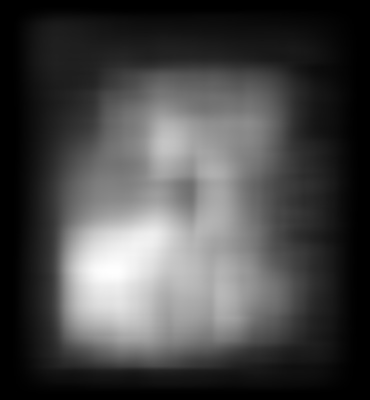
\includegraphics[width=0.6in,height=0.8in]{./Figures/previews/CSH.jpg} 
    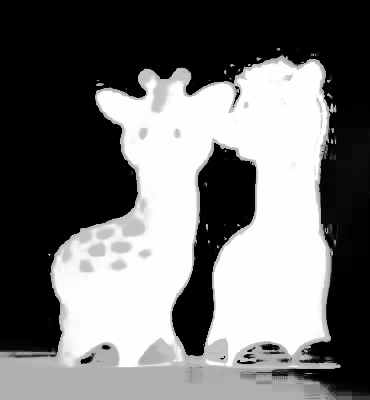
\includegraphics[width=0.6in,height=0.8in]{./Figures/previews/CSD.jpg} 
    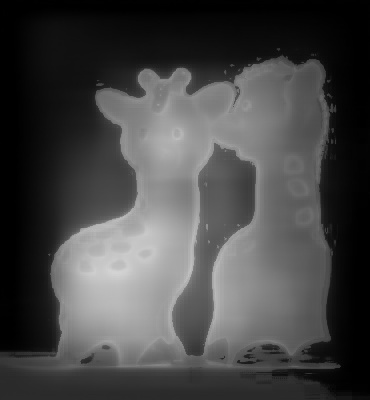
\includegraphics[width=0.6in,height=0.8in]{./Figures/previews/Composed.jpg} \\
    {\footnotesize Fig.3 Original Image and Preview of feature maps \\ 
       Left to Right: (b) multiscale contrast  (c) center surround histogram \\[-1mm] 
    (d) color spatial distribution (e) composed unary potential}
    \end{center}
    The value of each feature $F_k(a_x,I)$ comes from a normalised feature map $f_k(x,I)\in[0,1]$, and for each pixel:
    $$
    F_k(a_x,I) = \left\{\begin{matrix}f_k(x,I), & a_x=0\\1-f_k(x,I), & a_x=1\end{matrix}\right. 
    $$
%}}}

%% Feature Extraction (2 pages)
\section{Feature Extraction}
Feature Extraction, widely acknowledged as the most significant component of computer vision task,
represents how we want the computer to interpret the raw iamges. In this project, we just focus
on three critical features, each of which is capable of capturing the saliency individually but
in various level of scope. They are respectively Multiscale Contrast, Center Surround Histogram 
and Color Spatial Distribution. 
\subsection{Multiscale Contrast}
Constrast is commonly utilised as local feature because the contrast operator simulates
the human visual receptive fields. Specifically, it captures the point that salient object
tends to have tremendous contrast to the surroundings in its boundary (not vice versa).
Since we may have no preknowledge about the size of salient object, it is usual
to compute the contrast at multiple scale. 

    \begin{center}    
        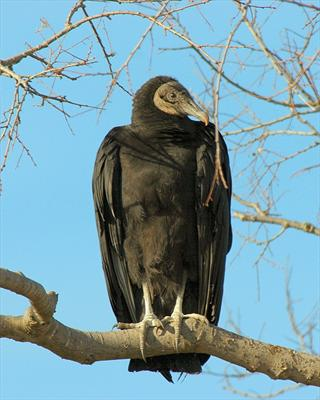
\includegraphics[width=0.65in,height=0.9in]{./Figures/pyramid/5_145_145839raw.jpg} \hspace{2mm}
    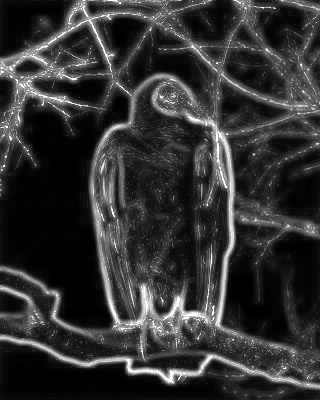
\includegraphics[width=0.65in,height=0.9in]{./Figures/pyramid/5_145_145839_p0.jpg} 
    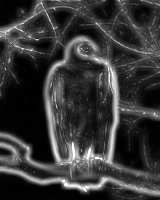
\includegraphics[width=0.325in,height=0.45in]{./Figures/pyramid/5_145_145839_p1.jpg} 
    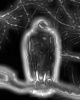
\includegraphics[width=0.1625in,height=0.225in]{./Figures/pyramid/5_145_145839_p2.jpg} 
    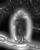
\includegraphics[width=0.08125in,height=0.1125in]{./Figures/pyramid/5_145_145839_p3.jpg} 
    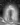
\includegraphics[width=0.040625in,height=0.0575in]{./Figures/pyramid/5_145_145839_p4.jpg} 
    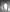
\includegraphics[width=0.0203125in,height=0.02825in]{./Figures/pyramid/5_145_145839_p5.jpg} \hspace{1mm}
    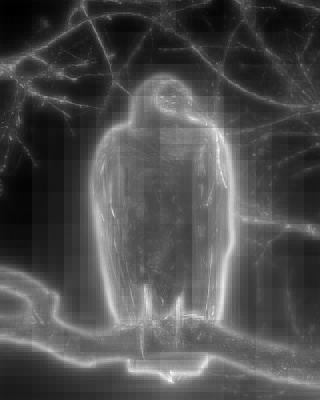
\includegraphics[width=0.65in,height=0.9in]{./Figures/pyramid/5_145_145839.jpg} \\
    \footnotesize Fig. Pyramid of Multiscale Contrast.  \\
    (a) leftmost: Original Image. (b) rightmost: Multiscale Feature Map. \\
    (c) immediate images: multiscale pyramids from level $1$ to $6$.
    \end{center}

Hence, define the multiscale constrast to be 
a contrast map from the linear combination of image contrast at all levels of an N-level
gaussian image pyramid, using the pixels $x$ in the image $I$:
    $$
    f_c(x,I) = \SUM_{n = 1}^{N}\SUM_{x'\in W(x)}||I^n(x)-I^n(x')||^2
    $$
where W(x) is a window that delineates which area to consider for neighbouring pixels to compare contrast values.

% TODO add explanation for why we need to choose such window size and pyramid level.
In our implementation, we choose the total number of pyramid level $N$ to be $6$ and 
the size of the window to be $9 \times 9$. 

    \begin{center}
    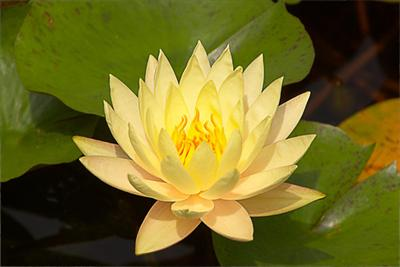
\includegraphics[width=0.7in,height=0.54in]{./Figures/contrast/1orig.jpg}
    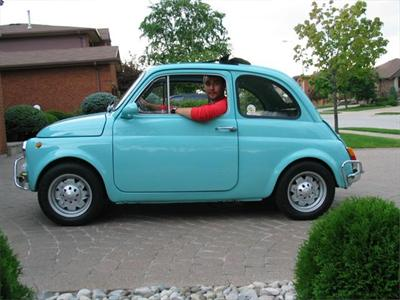
\includegraphics[width=0.7in,height=0.54in]{./Figures/contrast/2orig.jpg}
    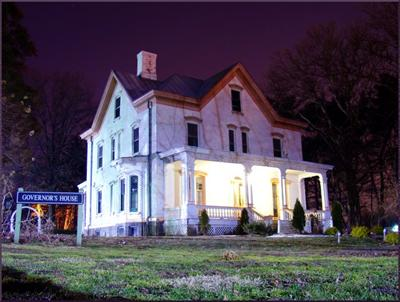
\includegraphics[width=0.7in,height=0.54in]{./Figures/contrast/3orig.jpg}
    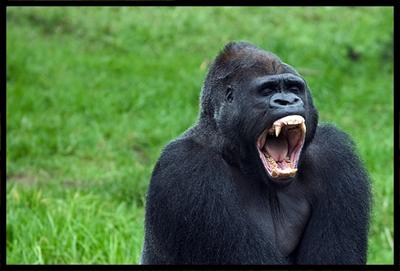
\includegraphics[width=0.7in,height=0.54in]{./Figures/contrast/4orig.jpg}\\
    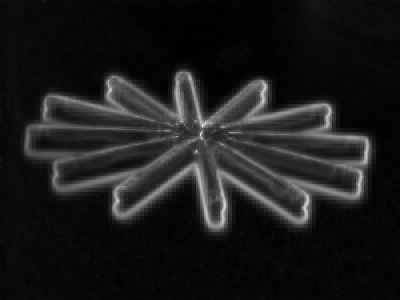
\includegraphics[width=0.7in,height=0.54in]{./Figures/contrast/1cont.jpg}
    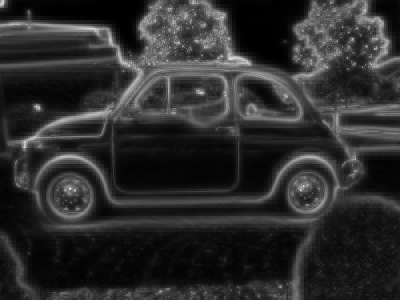
\includegraphics[width=0.7in,height=0.54in]{./Figures/contrast/2cont.jpg}
    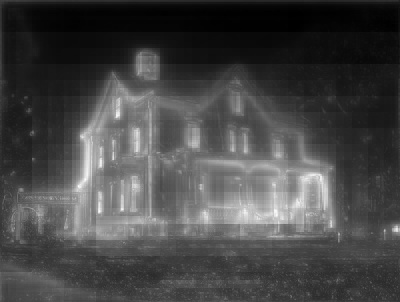
\includegraphics[width=0.7in,height=0.54in]{./Figures/contrast/3cont.jpg}
    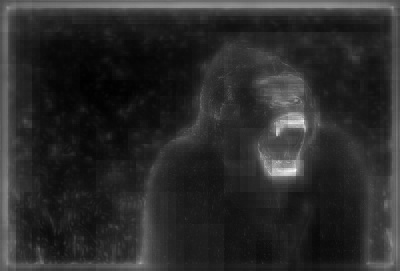
\includegraphics[width=0.7in,height=0.54in]{./Figures/contrast/4cont.jpg}\\
    \footnotesize Fig. Local Feature: Multiscale Contrast under various scenes
    \end{center}

It is evident that the Multiscale Contrast give high distinction between the boundary and non-boundary region. 
This provides us a precise description of where the boundary of salient object exist in the output binary mask.

But there are also some drawbacks. First and foremost, boundary of objects are highlighted, which are not desired.
We only wish to label, at most, the boundary of salient object, rather thatn all boundaries in one image. 
This may possibly lead to some "saliency leak" in the ultimate result and deteriorate detection precision.
Furthermore, the pixels within the salient objects are usually ignored in the sense that 
usually the salient object has low contrast within its body.
\subsection{Center Surround Histogram}

\subsection{Color Spatial Distribution}
    Create a Gaussian Mixture Model to compute the spatial variance and continuity of colour in an image.

    The component model is created from only a subset of the pixels in the image, and the maximum number of iterations is limited in order to reduce the time taken to compute this feature without sacrificing too much accuracy.

    \begin{center}
    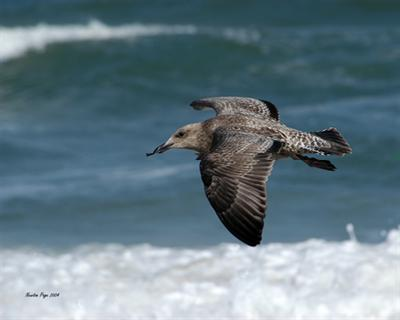
\includegraphics[width=0.72in,height=0.52in]{./CSD_image/1.jpg}
    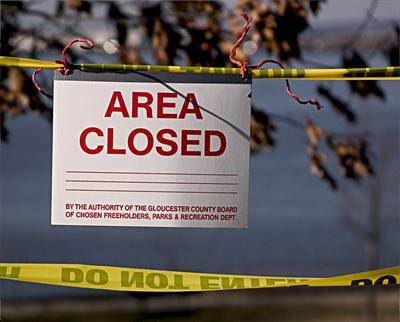
\includegraphics[width=0.72in,height=0.52in]{./CSD_image/2.jpg}
    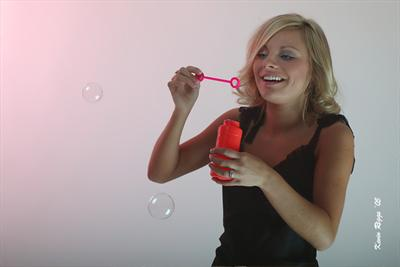
\includegraphics[width=0.72in,height=0.52in]{./CSD_image/3.jpg}\\
    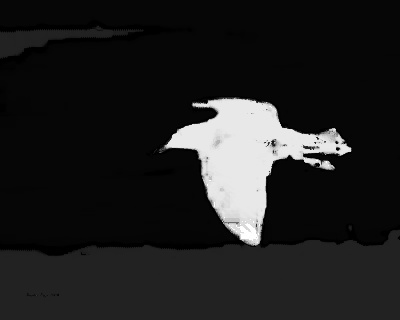
\includegraphics[width=0.72in,height=0.52in]{./CSD_image/1_CSD.jpg}
    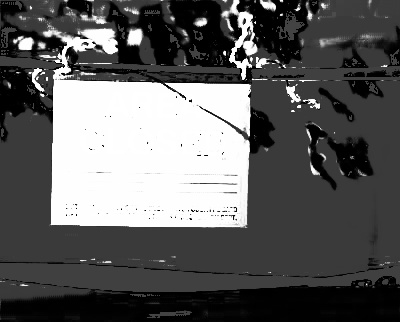
\includegraphics[width=0.72in,height=0.52in]{./CSD_image/2_CSD.jpg}
    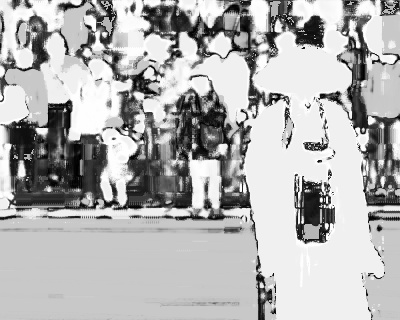
\includegraphics[width=0.72in,height=0.52in]{./CSD_image/3_CSD.jpg} \\
    \footnotesize Fig. 
    \end{center}

    Each pixel is associated to a colour component with the probability
    $$
    P(c|I_x) = \frac{\omega_c\mathcal{N}(I_x|\mu_c,\sigma_c)}{\SUM_c \omega_c \mathcal{N}(I_x|\mu_c,\Sigma_c)}
    $$
    where $\omega_c$ is the weight, $\mu_c$ is the mean colour, $\sigma_c$ is the covariance, and $\mathcal N(I_x|\mu_c,\sigma_c)$ is the multivariate normal distribution of the $c^{th}$ component.

    The final colour spatial distribution feature is defined as a weighted sum:
    $$
    f_s(x,I)\propto\SUM_c p(c|I_x)\cdot(1-V(c))
    $$
    where $V(c)$ is the normalised covariance (horizontal and vertical variances) of the $c^{th}$ component, contained between 0 and 1.
%% Learning (0.5 page)
\section{Learning}

%% CRF Inference (0.5 page)
\section{CRF Inference}

%% Pixel Level result presentation (1 page)
\section{Result Presentation}

%% Result evaluation in rectangle level (1 page)
\section{Evaluation}

%% Discussion (existing flaws and possible improvements) (0.5 page)
\section{Discussion}
\subsection{Current Weaknesses}
\subsection{Possible Improvement}

%% acknowlegement and reference (0.5 page)
\begin{thebibliography}{99} \fontsize{9pt}{50} \setlength{\itemsep}{-0.5pt} 
    \bibitem 1 Liu, Tie, et al. "Learning to detect a salient object." 
        \textit{Computer Vision and Pattern Recognition, 2007. CVPR07. IEEE Conference on. IEEE, 2007}.

    \bibitem 2 Liu, Tie, et al. "Learning to detect a salient object." 
        \textit{Pattern Analysis and Machine Intelligence, IEEE Transactions on 33.2 (2011): 353-367}. 

    \bibitem 3 Itti, Laurent, Christof Koch, and Ernst Niebur. "A model of saliency-based visual attention for rapid scene analysis."
        \textit{Pattern Analysis and Machine Intelligence, IEEE Transactions on 20.11 (1998): 1254-1259}.

    \bibitem 4 Ma, Yu-Fei, and Hong-Jiang Zhang. "Contrast-based image attention analysis by using fuzzy growing."
        \textit{ Proceedings of the eleventh ACM international conference on Multimedia. ACM, 2003}. 

    \bibitem 5 Gould, Stephen. "DARWIN: A Framework for Machine Learning and Computer Vision Research and Development." 
        \textit{Journal of Machine Learning Research 13 (2012): 3533-3537}

\end{thebibliography}
%-------------------------------------------------------------------------

\end{document}

